\begin{block}{Results}
  \begin{figure}
    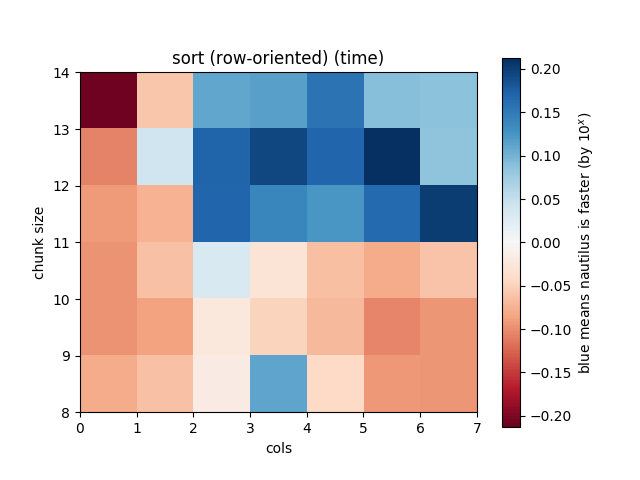
\includegraphics[height=30cm]{plots/sort_2d.png}
    \caption{~Performance in Nautilus and Linux wihle varying the parameters of the database (number of columns and chunk-size).}
    \label{fig:sort_2d}
  \end{figure}

  We see that for certain workloads, usually when the database size is large, Nautilus outperforms Linux. This is because Nautilus has larger page size and incurs less TLB misses. See Table \ref{table:cache_miss}.

  \begin{figure}
    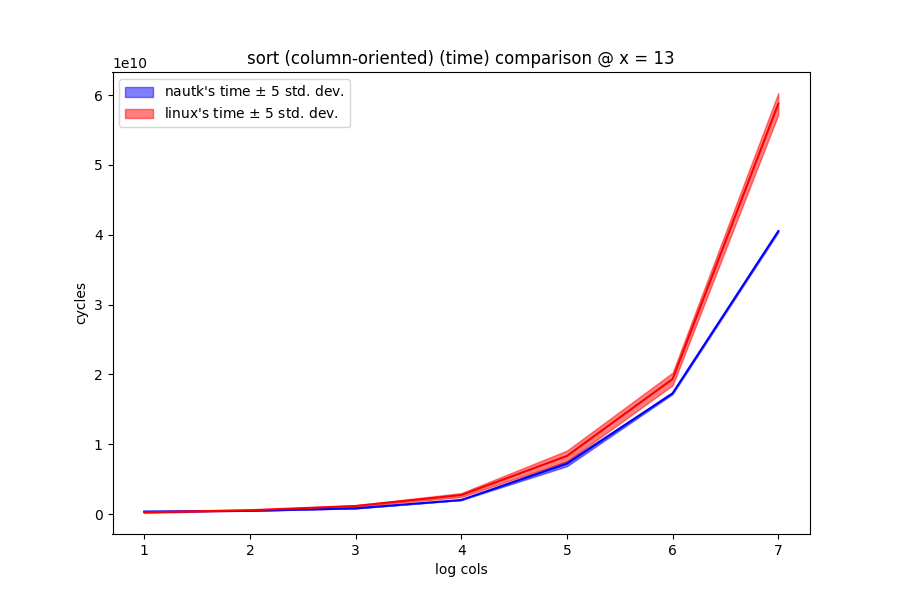
\includegraphics[height=30cm]{plots/sort.png}
    \caption{~Performance viewed with uncertainty with a fixed chunk size, varying the number of columns.}
    \label{fig:sort}
  \end{figure}

  Furthermore, we see that Nautilus has more consistent runtimes than Linux. This effect is observed even when Linux outperforms Nautilus. This is because Nautilus does not have scheduling interrupts, so it avoids unpredictable detours. See Table \ref{table:cache_miss}.

  \begin{figure}
    \begin{table}
      \begin{tabular}{l || c | c }
        Operation  & Linux & Nautilus \\
        \hline\hline
        TLB misses               & 8e6 & 1e6 \\
        Instruction cache misses & 2e6 & 0e6  \\

        % I don't have perf-counter data for the following
        % (there is no perf counter)
%        Page faults              &     & 0 \\
%        Context switches         &     & 0 \\
%        Interrupts               &     & 0 \\
      \end{tabular}
      \label{table:cache_miss}
      \caption{~Performance metrics for running with a $2^7$ columns and $2^13$ chunk size.}
    \end{table}
  \end{figure}
\end{block}

%%% Local Variables:
%%% mode: latex
%%% TeX-master: "main"
%%% End:
